\documentclass[final]{beamer}

% =========================================================
% Preamble - Load all settings from separate files
% =========================================================
% =========================================================
% Packages and Theme Setup
% =========================================================
\usepackage[orientation=landscape,size=a0,scale=1.0,debug]{beamerposter}
\usepackage{graphicx}
\usepackage{booktabs}
\usepackage{amsmath}
\usepackage{amssymb}
\usepackage{array}
\usepackage{colortbl}
\usepackage{multicol}
\usepackage{tikz}
\usetikzlibrary{shapes,arrows,positioning}

% Theme Choice - Using "default" to allow custom headers
\mode<presentation>{\usetheme{default}}

% =========================================================
% Font Settings - Arial-like (Helvetica)
% =========================================================
\usepackage[T1]{fontenc}
\usepackage{helvet}
\renewcommand{\familydefault}{\sfdefault}

% Block title font
\setbeamerfont{block title}{size=\Large,series=\bfseries}

% =========================================================
% Colors - Professional Academic Palette
% =========================================================
\definecolor{HKUGreen}{RGB}{0, 98, 73}        % HKU Green for headers
\definecolor{AccentGold}{RGB}{180, 141, 61}    % Gold accent
\definecolor{DarkSlate}{RGB}{47, 62, 70}       % Dark text
\definecolor{LightBg}{RGB}{248, 249, 250}      % Light background for blocks
\definecolor{MediumGray}{RGB}{108, 117, 125}   % Secondary text
\definecolor{AlertRed}{RGB}{192, 57, 43}       % For emphasis

% Beamer Color Settings
\setbeamercolor{headline}{bg=HKUGreen,fg=white}
\setbeamercolor{block title}{bg=HKUGreen,fg=white}
\setbeamercolor{block body}{bg=LightBg,fg=DarkSlate}
\setbeamercolor{itemize item}{fg=AccentGold}
\setbeamercolor{enumerate item}{fg=AccentGold}
\setbeamercolor{itemize subitem}{fg=HKUGreen}

% Remove default beamer margins
\setbeamersize{text margin left=1cm, text margin right=1cm}

% =========================================================
% Custom Headline Template
% =========================================================
\setbeamertemplate{headline}{
  \leavevmode
  \vskip-3pt
  \begin{beamercolorbox}[wd=\paperwidth,ht=7cm,dp=0.3cm,leftskip=1cm,rightskip=1cm]{headline}
    \vskip0.4cm
    \begin{columns}[c]
      % Left Column: Conference Logo/Name
      \begin{column}{.12\paperwidth}
        \centering
        {\fontsize{32}{36}\selectfont \textbf{TRB 2026}}\\[0.2cm]
        {\Large Annual Meeting}\\[0.1cm]
        {\large Washington, D.C.}
      \end{column}
      
      % Center Column: Title and Authors
      \begin{column}{.76\paperwidth}
        \centering
        {\fontsize{52}{58}\selectfont \textbf{Repositioning in Bike Sharing Systems with}}\\[0.3cm]
        {\fontsize{52}{58}\selectfont \textbf{Broken Bikes Considering On-site Repairs}}\\[0.5cm]
        {\Large Runqiu Hu$^{1}$, W.Y. Szeto$^{1,2,3}$, Sin C. Ho$^{4}$}\\[0.3cm]
        {\normalsize $^{1}$Dept. of Civil Engineering, HKU \quad 
        $^{2}$HKU Shenzhen Institute of Research and Innovation \quad
        $^{3}$GD-HK-Macau Joint Lab for Smart Cities \quad
        $^{4}$CUHK}
      \end{column}
      
      % Right Column: Paper Info
      \begin{column}{.12\paperwidth}
        \centering
        {\normalsize \textbf{Transportation Research}}\\
        {\normalsize \textbf{Part E} (2025)}\\[0.2cm]
        {\small DOI: 10.1016/j.tre.2025.104155}
      \end{column}
    \end{columns}
    \vskip0.2cm
  \end{beamercolorbox}
  
  % Gold accent line below header
  \begin{beamercolorbox}[wd=\paperwidth,ht=0.25cm]{accent}
    {\color{AccentGold}\rule{\paperwidth}{0.25cm}}
  \end{beamercolorbox}
}

% Remove default footline
\setbeamertemplate{footline}{}

% Remove navigation symbols
\setbeamertemplate{navigation symbols}{}


% =========================================================
% Document Body - Redesigned for clarity and visual flow
% Following TRB Poster Guidelines: 3-4 main concepts,
% 50% text / 50% graphics, clear left-to-right flow
% =========================================================
\begin{document}
\begin{frame}{}
    \vspace{-0.5cm}
    
    % Three Column Layout with clear narrative flow
    \begin{columns}[t]
        
        % ---------------------------------------------------------
        % COLUMN 1: THE PROBLEM (Why does this matter?)
        % ---------------------------------------------------------
        \begin{column}{0.31\paperwidth}
            
            % Section 1: Problem Overview - THE CHALLENGE
% Clear, visual introduction to the problem
\begin{block}{\Large The Challenge: Bike Sharing Operations}
    
    \vspace{0.2cm}
    \begin{columns}[c]
        \begin{column}{0.48\linewidth}
            \centering
            \textbf{\textcolor{AlertRed}{Demand Imbalance}}\\[0.2cm]
            % PLACEHOLDER: Add illustration showing empty/full stations
            \fbox{\parbox{0.9\linewidth}{\centering\vspace{0.6cm}
            \textit{[Placeholder: Illustration of stations becoming empty or full during peak hours]}
            \vspace{0.6cm}}}
            \\[0.2cm]
            {\small Stations become empty or full}\\
            {\small $\rightarrow$ Users cannot pick up/return bikes}
        \end{column}
        \begin{column}{0.48\linewidth}
            \centering
            \textbf{\textcolor{AlertRed}{Broken Bikes}}\\[0.2cm]
            \includegraphics[width=0.85\linewidth]{figures/two-repair-modes.png}
            \\[0.2cm]
            {\small Barcelona: 67\% bikes damaged}\\
            {\small NYC: 2\% need daily repairs}
        \end{column}
    \end{columns}
    
    \vspace{0.3cm}
    \begin{center}
        \colorbox{AccentGold!20}{\parbox{0.9\linewidth}{\centering
        \textbf{Current solutions use trucks to relocate bikes between stations.}\\[0.1cm]
        But what about \textbf{repairing bikes on-site}?
        }}
    \end{center}
    
\end{block}

            \vspace{0.2cm}
            
            % Section 2: Research Gap - WHY THIS MATTERS
\begin{block}{\Large Research Gap \& Our Question}
    
    \vspace{0.2cm}
    \textbf{Existing Studies Focus On:}
    \begin{itemize}
        \item[$\checkmark$] Truck-based bike repositioning
        \item[$\checkmark$] Moving broken bikes to repair depots
        \item[$\times$] \textcolor{MediumGray}{On-site repairs by dedicated repairers}
    \end{itemize}
    
    \vspace{0.3cm}
    \begin{center}
        \colorbox{HKUGreen!15}{\parbox{0.95\linewidth}{\centering
        \vspace{0.2cm}
        {\Large \textbf{Research Question}}\\[0.2cm]
        {\normalsize How can we \textbf{jointly optimize} truck repositioning}\\
        {\normalsize and \textbf{on-site bike repairs} to improve service quality?}\\[0.1cm]
        \vspace{0.1cm}
        }}
    \end{center}
    
    \vspace{0.3cm}
    \centering
    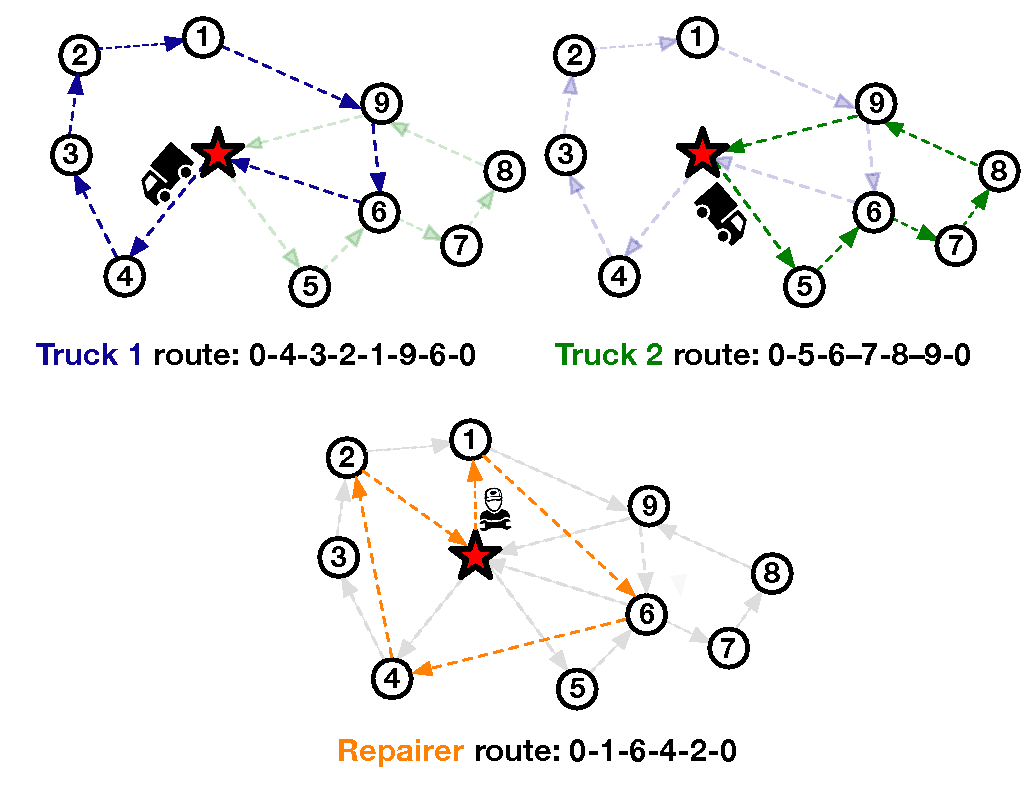
\includegraphics[width=0.92\linewidth]{figures/add_repairer.pdf}
    
    \vspace{0.15cm}
    {\small \textbf{Our integrated system:} Trucks (blue routes) relocate bikes while repairers (dashed routes) fix bikes on-site.}
    
\end{block}

            
        \end{column}

        % ---------------------------------------------------------
        % COLUMN 2: THE SOLUTION (What did we do?)
        % ---------------------------------------------------------
        \begin{column}{0.31\paperwidth}
            
            % Section 3: Our Approach - THE SOLUTION
\begin{block}{\Large Our Approach}
    
    \vspace{0.2cm}
    \textbf{We developed two solution methods:}
    
    \vspace{0.3cm}
    \begin{columns}[t]
        \begin{column}{0.48\linewidth}
            \centering
            \colorbox{HKUGreen!10}{\parbox{0.95\linewidth}{
            \vspace{0.2cm}
            \centering
            \textbf{Exact Method}\\[0.1cm]
            {\small Mathematical Optimization}\\[0.2cm]
            \begin{itemize}
                \item Time-indexed model
                \item Tracks bikes \& repairers
                \item Minimizes dissatisfaction
            \end{itemize}
            \vspace{0.1cm}
            {\footnotesize \textcolor{MediumGray}{For small networks (< 50 stations)}}
            \vspace{0.1cm}
            }}
        \end{column}
        \begin{column}{0.48\linewidth}
            \centering
            \colorbox{AccentGold!15}{\parbox{0.95\linewidth}{
            \vspace{0.2cm}
            \centering
            \textbf{Fast Algorithm}\\[0.1cm]
            {\small Hybrid Genetic Search}\\[0.2cm]
            \begin{itemize}
                \item Scales to 500+ stations
                \item Smart time allocation
                \item Near-optimal solutions
            \end{itemize}
            \vspace{0.1cm}
            {\footnotesize \textcolor{MediumGray}{For real-world city networks}}
            \vspace{0.1cm}
            }}
        \end{column}
    \end{columns}
    
    \vspace{0.3cm}
    \centering
    \includegraphics[width=0.92\linewidth]{figures/fig_3_2_temporal_illustration.png}
    
    \vspace{0.15cm}
    {\small \textbf{How it works:} The model tracks bike inventory changes over time as trucks and repairers visit stations.}
    
\end{block}

            \vspace{0.2cm}
            
            % Section 4: Key Innovation - WHAT'S NEW
\begin{block}{\Large Key Innovation: Smart Time Allocation}
    
    \vspace{0.2cm}
    \textbf{The Problem:} Spending too much time at early stations leaves no time for later ones.
    
    \vspace{0.25cm}
    \textbf{Our Solution: Station Budget Constraint}
    \begin{itemize}
        \item Each station gets a \textbf{time budget} based on its potential benefit
        \item Stations with more broken bikes get more time
        \item Unused time \textbf{redistributed} to later stations
    \end{itemize}
    
    \vspace{0.25cm}
    \centering
    \includegraphics[width=0.92\linewidth]{figures/fig_4_1_bcrf_illustration.png}
    
    \vspace{0.2cm}
    {\small \textbf{Prioritizing stations:} Heatmaps show dissatisfaction levels. Darker colors = higher priority for service.}
    
    \vspace{0.25cm}
    \begin{center}
        \colorbox{AccentGold!20}{\parbox{0.9\linewidth}{\centering
        \vspace{0.15cm}
        \textbf{Result:} Better service across all stations, not just the first few.
        \vspace{0.15cm}
        }}
    \end{center}
    
\end{block}

            
        \end{column}

        % ---------------------------------------------------------
        % COLUMN 3: THE IMPACT (What did we find?)
        % ---------------------------------------------------------
        \begin{column}{0.31\paperwidth}

            % Section 5: Results - WHAT DID WE FIND
\begin{block}{\Large Results: Algorithm Performance}
    
    \vspace{0.2cm}
    \textbf{Comparison with Commercial Solver (Gurobi):}
    
    \vspace{0.2cm}
    \centering
    \includegraphics[width=0.92\linewidth]{figures/table_5_4_results.png}
    
    \vspace{0.25cm}
    \begin{columns}[c]
        \begin{column}{0.48\linewidth}
            \centering
            \colorbox{HKUGreen!15}{\parbox{0.9\linewidth}{\centering
            \vspace{0.2cm}
            {\LARGE \textbf{4--33\%}}\\[0.1cm]
            {\small Better solution quality}\\
            {\footnotesize (lower user dissatisfaction)}
            \vspace{0.2cm}
            }}
        \end{column}
        \begin{column}{0.48\linewidth}
            \centering
            \colorbox{AccentGold!20}{\parbox{0.9\linewidth}{\centering
            \vspace{0.2cm}
            {\LARGE \textbf{6--51 sec}}\\[0.1cm]
            {\small vs. 2 hours+}\\
            {\footnotesize Computation time}
            \vspace{0.2cm}
            }}
        \end{column}
    \end{columns}
    
    \vspace{0.3cm}
    \begin{center}
        {\normalsize \textbf{Scales to real cities:} Tested on networks with up to \textbf{500 stations}}\\[0.1cm]
        {\small (Gurobi fails for networks larger than 200 stations)}
    \end{center}
    
\end{block}

            \vspace{0.2cm}

            % Section 6: Takeaways - PRACTICAL IMPACT
\begin{block}{\Large Practical Takeaways for Operators}
    
    \vspace{0.2cm}
    \textbf{When should you deploy on-site repairers?}
    
    \vspace{0.2cm}
    \begin{columns}[c]
        \begin{column}{0.48\linewidth}
            \centering
            \includegraphics[width=0.9\linewidth]{figures/cost_effectiveness_l30.jpeg}
            \\[0.1cm]
            {\footnotesize 30\% broken bikes}
        \end{column}
        \begin{column}{0.48\linewidth}
            \centering
            \includegraphics[width=0.9\linewidth]{figures/cost_effectiveness_l50.jpeg}
            \\[0.1cm]
            {\footnotesize 50\% broken bikes}
        \end{column}
    \end{columns}
    
    \vspace{0.25cm}
    \colorbox{AlertRed!15}{\parbox{0.95\linewidth}{
    \vspace{0.15cm}
    \centering
    \textbf{Key Decision Rules:}
    \begin{itemize}
        \item \textbf{< 20\% broken:} Trucks alone sufficient
        \item \textbf{> 30\% broken:} On-site repairers cost-effective
        \item \textbf{Repair time > 11 min:} Never cost-effective
    \end{itemize}
    \vspace{0.1cm}
    }}
    
    \vspace{0.25cm}
    \begin{center}
        \colorbox{HKUGreen!15}{\parbox{0.95\linewidth}{\centering
        \vspace{0.1cm}
        {\normalsize \textbf{Bottom Line:} Invest in preventive maintenance to keep repair times low.}
        \vspace{0.1cm}
        }}
    \end{center}
    
    \vspace{0.2cm}
    \hrule
    \vspace{0.2cm}
    
    % References and Contact
    \begin{columns}[c]
        \begin{column}{0.62\linewidth}
            {\footnotesize \textbf{Reference:} Hu, R., Szeto, W.Y., \& Ho, S.C. (2025). Repositioning in bike sharing systems with broken bikes considering on-site repairs. \textit{Transportation Research Part E}, 104155.}
            
            \vspace{0.1cm}
            {\footnotesize \textbf{Acknowledgments:} NSFC (71771194), RGC Hong Kong (17206322)}
        \end{column}
        \begin{column}{0.33\linewidth}
            \centering
            % PLACEHOLDER: QR Code for paper
            \fbox{\parbox{0.7\linewidth}{\centering\vspace{0.5cm}
            \textit{[QR Code]}\\
            \textit{Scan for paper}
            \vspace{0.5cm}}}
            \\[0.1cm]
            {\footnotesize DOI: 10.1016/j.tre.2025.104155}
        \end{column}
    \end{columns}
    
\end{block}


        \end{column}
    \end{columns}
\end{frame}
\end{document}
